%! Author = rickr
%! Date = 11/27/2021
\subsection{The Ising Model}
In ideal \textit{paramagnetism} (magnetism where materials are weakly attracted by an external magnetic field) microscopic magnetic dipole moments respond only to an external field. 
However, in the real world, neighboring atomic dipoles are influenced by each other. 
When neighboring dipoles align parallel, even in the absence of an external field, we call the material a ferromagnet. 
The Ising model is a mathematical model used to describe ferromagnetism in terms of statistical mechanics. The model consists of discrete variables that represent the magnetic dipole moments of atomic spins and can have a value of $\pm 1$. 
The variables are used to describe preference for neighboring dipoles to align parallel or anti-parallel to each other \cite{schroeder2011thermal}.
\begin{figure}[h]
	\begin{center}
		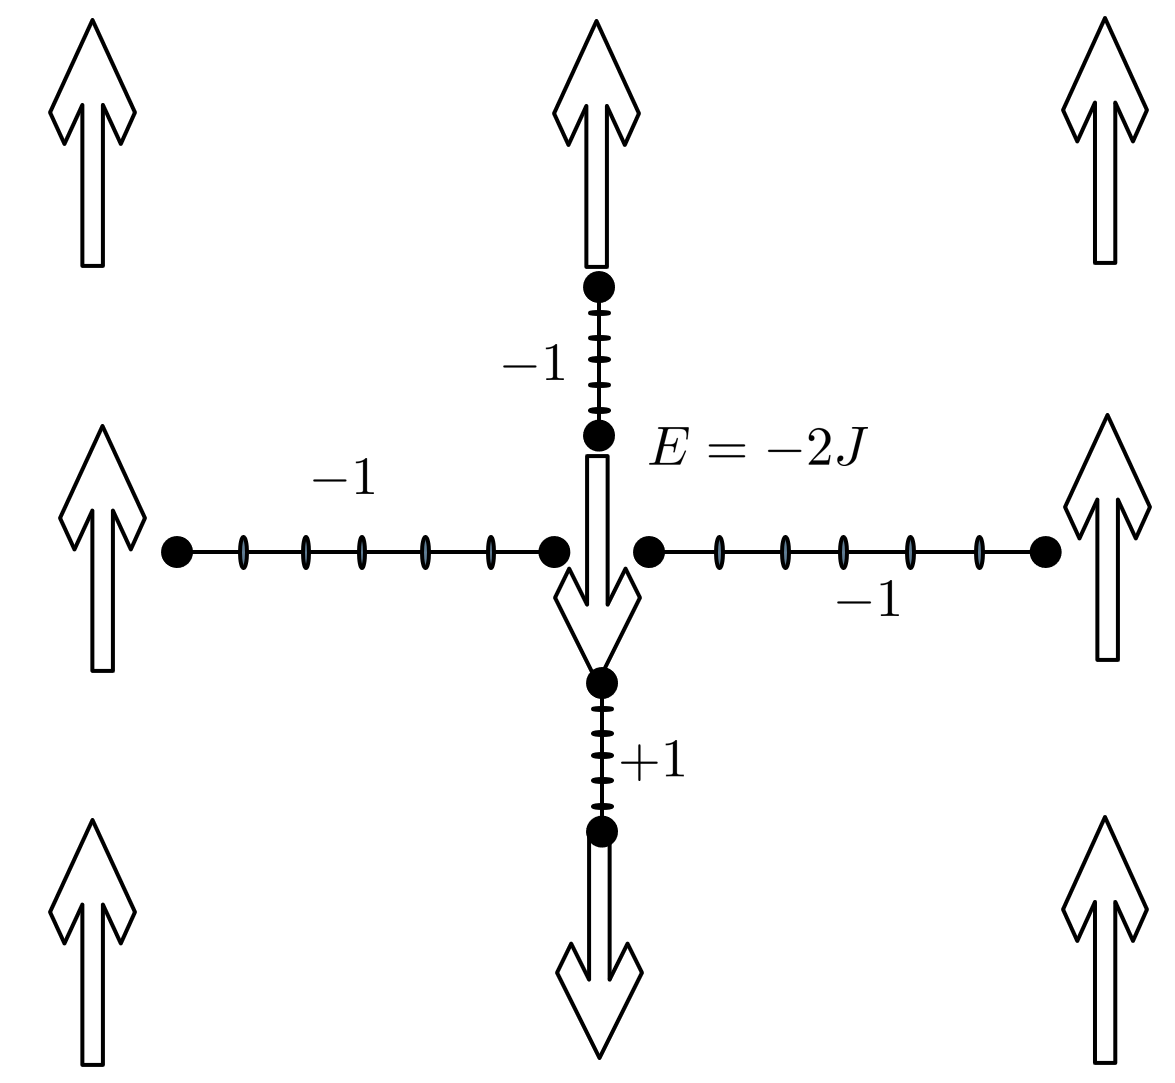
\includegraphics[width=4cm]{images/lattice}
	\end{center}
	\caption{\doublespacing Atomic spin states arranged into a 2-dimensional lattice structure under periodic boundary conditions. The energy of the particle at lattice site $k$ has a value $E = -2J$ and the total energy of the system is found by summing over the entire structure.}
	\label{fig:lattice}
\end{figure}

For example, consider a lattice of particles as shown in Figure \ref{fig:lattice}. 
Each particle has an associated spin state that can take the orientations of spin-up $|+\rangle$ or spin-down $|-\rangle$ with values $\sigma_k = +1$ and $\sigma_k = -1$ respectively. The energy associated with the particle at lattice site $k$ is found to be 
\begin{equation}
	E_k= - J\sum_{<i,j>}\sigma_k^i\sigma_k^j \quad \cite{ising1925beitrag}
	\label{eq:latticeSiteEnergy}
\end{equation}
where $J$ is a coupling constant, $\sigma_k$ is a discrete variable, and $<i,j>$ means to sum over the nearest neighbors. Note that for parallel spins, $J>0$, for anti-parallel spins $J<0$, and for no interaction $J = 0$. 
In the presence of a magnetic field $\vec{B}$, the kinetic and potential energy of the system can be represented by the Hamiltonian
\begin{equation}
	H_0 = \frac{g_s}{2}\mu_B B\sum_{i=1}^N \sigma_z^i - J\sum_{<i,j>}\sigma_z^i\sigma_z^j
	\label{eq:isingHamiltonian}
\end{equation} 
where the spin g-factor for an electron $g_s$ and the Bohr magneton $\mu_B$ are constants, and the discrete variable $\sigma_k$ has been replaced with the Pauli z-operator $\sigma_z$ as in Equation \ref{eq:transformation}. 
There are many techniques for solving generalized Ising models including transfer matrix methods\cite{onsager1944crystal}, graphical/combinatorial methods\cite{feynman1972statistical}, and Monte Carlo simulations\cite{schroeder2011thermal}. 
However, with the advent of quantum computation, the time independent Schrodinger equation is especially convenient.